\section{Baseline}
\label{CHAPTER_BaselineDev}

\subsection{Feature Selection}
\label{SUBSECTION_FeatureSelection}
In this section, we describe a really important part of the development of our solution, which is the feature selection \footnote{Refer to: \texttt{Task02\_SupervisedLearning\_Baseline\_Barba\_Guerrero\_Schmidt.ipynb}.}. Although we performed feature selection in an incremental way, we decided to group all the different improvements performed on the feature selection, from scratch until the last version of the feature selection used in the final solution.

Essentially, we first used all the features to obtain an initial result, to gain some understanding of how important feature selection was going to be. As the result felt miserable, we decided to perform feature selection, which was first performed using domain knowledge, and it was later improved by making use of decision trees, which allowed us to gain information on the relevance of the features themselves.


\subsubsection{Feature Selection using Domain Knowledge}
\label{SUBSUBSECTION_FeatureSelectionDomainKnowledge}
The first step in order to improve the results was to perform an in-depth read of the different features. Their description can be found in the challenge’s website \cite{DrivenData22}. As a result of an initial analysis, it was decided to keep the following characteristics:
\begin{itemize}
    \item \texttt{age}: we understood that the age of the building would have an impact in its damage degree. Thus, we decided to include it.
    \item  \texttt{area\_percentage}: we considered that the damage degree of a building somehow depended on how big the building was. Thus, we also included this characteristic.
    \item Variables related to the building material were also included, e.g. \texttt{has\_superstructure\_adobe\_mud}, \texttt{has\_superstructure\_mud\_mortar\_stone}, \texttt{has\_superstructure\_stone\_flag}. The reason why they were included is that, using domain knowledge, we can understand that the material must have a real impact when determining the damage degree of the building, thus it was also included.
    \item \texttt{geo\_level\_x\_id}: the 3 variables associated with the location of the building were also added. This is because we understood that the distance from the earthquake’s epicentre could play an important role when determining the damage degree of the building.
\end{itemize}

As a result of this domain-knowledge-based feature selection, we obtained a direct impact in the different algorithms, thus proving that feature selection is key to maximize the performance of our classifier.

\subsubsection{Feature Selection using Decision Trees}
\label{SUBSUBSECTION_FeatureSelectionDTs}

As we’ve learned from the lectures, implementations of decision tree classifiers will order each feature, and therefore a decision, based on its importance and amount of information to be gained from making it. More specifically, the most important decisions will be made in a lower depth of the tree, reducing the overall amount of decisions that have to be made. After a decision tree classifier has been trained, the feature importance list can simply be exported and used for analysis and feature selection purposes.

It is important to note that we preprocess the input dataset to the classification process using the OneHot-Encoding for compatibility reasons, rolling out the amount of features from 38 to 68. In a first attempt of narrowing down the most important features using decision trees, we started training the classifier algorithms with the feature selection from our previous step already applied. Therefore, the amount of input features to the classifier is 17. By doing this, we were able to further decrease the amount of input features by eliminating those which don’t contribute much information value.

However, thanks to the feedback provided, performing a feature selection process before training the decision tree classifier turned out to be an unnecessary generalization. Assuming that we forgot an important feature in our preliminary feature selection using domain knowledge, we would not be able to detect this error. Furthermore, since the f1-score of the classifier itself does not turn out to be higher than other techniques in the baseline work, the feature selection from decision trees should be improved as much as possible. So, in a second attempt, the decision tree classifier is trained with all the 68 features. Figure \ref{PICTURE_featureimportances_dt} shows the feature importance of the twenty most relevant features. We decide to pick the seven most relevant features, which sum up to describe 85\% of the most important features of the dataset.

\begin{figure}[h!]
	\centering
            \includegraphicscentered{images/feature_importances_dt.png}{130mm}
	\caption{Plot of most important features, extracted from trained \texttt{DecisionTreeClassifier}.}
	\label{PICTURE_featureimportances_dt}
\end{figure}

Taking a look at the domain-based feature selection, we notice that the 4th most important feature “\texttt{foundation\_type\_r}”, which is a product of the OneHot-Encoding, was overlooked. We extract the seven most important features (see figure \ref{PICTURE_featureimportances_dt}), until \texttt{height\_percentage}, as the most important values to be used in our reduced set of features.

\subsection{Baseline Development}
In order to develop the baseline of the project, we decided to apply three simple algorithms to create initial classifiers that we could test to see how good or bad they perform\footnote{Refer to: \texttt{Task02\_SupervisedLearning\_Baseline\_Barba\_Guerrero\_Schmidt.ipynb}}. The baseline would be determined by the algorithm with the best performance in the competition, i.e. real data.

Thus, the idea is to obtain a baseline that can be improved with more complex algorithms to improve in a more fine-grained manner the performance of the classifier.

\subsubsection{Naive-Bayes}
The first algorithm that we used in order to obtain a classifier is Naive-Bayes. In this case, the algorithm does not require parametrization, thus its application is simpler when compared to other algorithms.

However, Naive-Bayes does have different possible models that can be used, and the model to choose greatly depends on the features that were selected. 

In our case, the first execution used all the different features and ComplementNB as a model. The reason why we decided to choose ComplementNB over the rest of the models is that we performed an exploratory data analysis that showed unbalanced data. ComplementNB is a good model when managing such data, thus it looked like a decent decision when it was performed. However, the result was not that good, as we only reached an f1-score of 0.2648 (which is actually worse than randomly determining the labels – 0.33).

As a result, we decided to apply improvements. The first improvement we came up with is to perform a smarter feature selection. Thus, it is here when we applied the domain-knowledge-based feature selection explained in section 2.1. With that feature selection, we applied again ComplementNB as the model to be used, obtaining an f1-score in the test dataset of 0.2561. 

That last result proved that using the ComplementNB model was not such a good choice, because although data selection seemed to be just fine, the results were in fact worse. If we pay attention to the domain-knowledge-based feature selection, we can easily check that almost all variables are categorical and actually binary variables. BernoulliNB is a model that is known for being most effective when working with binary variables, as a consequence, we chose to apply the Bernoulli NB model keeping the same feature selection.

This last improvement led to a model that provided an f1-score of 0.5690 on the test dataset and 0.5665 of the driven data competition, which was already a good starting point for our baseline.

\subsubsection{KNN}
The second classification algorithm used is KNN. Contrary to Naive-Bayes, this algorithm requires a bit of parametrization, which will be discussed in the following paragraphs.

Implementing a basic KNeighborsClassifier with a k value of 8, taken randomly, the result obtained in the competition is a huge 0.7013, which at first sight seems like a big improvement from the previous model. It is remarkable to say that the first version of our KNN model used the features obtained via domain knowledge.

The first parameter we decided to tune is the number of neighbours. For this purpose, the easiest way to do this is to use the model to predict the output label using different numbers of neighbours, and comparing the accuracy of those trials. We compared the accuracy of both uniform and inverse distance, obtaining the result shown in figure \ref{PICTURE_figure_knn_01}.

And, while the best decision could be choosing uniform and a number of neighbours of around 64, we know that, from our empirical observations, the optimal result is provided by using a value for k of 32. This could be most likely due to the phenomena of overfitting. With this change, we increase the accuracy up to 0.7060. Another change included in the model is the use of Manhattan distance instead of the default Euclidean distance, which is less appropriate for our model. Thus, the accuracy reaches 0.7121.

However, there are a couple more changes that can be included in our model:
Better feature selection: with the most important features obtained using decision trees, the accuracy of the model slightly raises to 0.7128.
Normalization of values: some numerical columns, such as the geo id columns, the age, or the area and height percentage, present disparate values that can be normalized to make every one of them fit in a range from 0 to 1. With this easily applied technique, we reach a final accuracy value of 0.7215, the highest obtained in our baseline, which makes us barely reach the top 1000 submissions.

Figure \ref{PICTURE_figure_knn_02} shows the confusion matrix of the last model.

\begin{figure}[h!]
  \begin{minipage}[b]{0.5\linewidth}
    \centering
    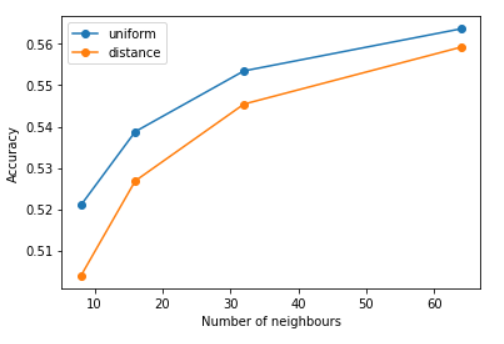
\includegraphics[width=60mm]{images/knn_figure_01.png}
    \caption{KNN: Manual tuning of parameters.}
    \label{PICTURE_figure_knn_01}
    \end{minipage}
  \hspace{0.1cm}
  \begin{minipage}[b]{0.5\linewidth}
    \centering
    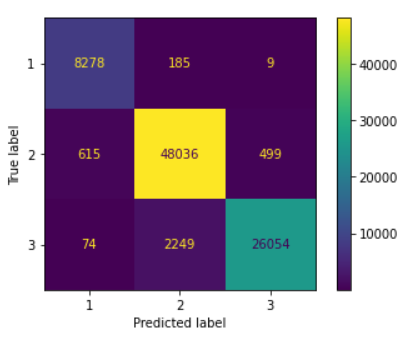
\includegraphics[width=55mm]{images/knn_figure_02.png}
    \caption{KNN: Confusion matrix.}
    \label{PICTURE_figure_knn_02}
  \end{minipage}
\end{figure}

As we can observe, our model is very robust at this point, but still fails to classify some 3rd grade earthquakes, as it considers them as 2nd grade, which is the main weakness the Naive-Bayes model also had.

\subsubsection{Decision Trees}

The third and last classification algorithm we applied to the dataset are decision trees. As already stated in the above section, the classifiers main advantages for this task are found in the feature selection capabilities, at least within the baseline step. In this section, we’ll be taking a closer look into the parametrization and training procedure for the decision tree classifier.

As mentioned, the classifier is trained with the full set of features of our dataset. As an initial step, we train the DecisionTreeClassifier without any parameters, which yields an f1-score of 0.6528, which is already a great result. However, it is not as good as the best f1-score we got from KNN.

For decision trees, we are able to make adjustments to the parameters \texttt{class\_weight}, \texttt{criterion}, \texttt{max\_depth}, \texttt{min\_samples\_split} and \texttt{min\_samples\_leaf}.
    
From the exploratory data analysis, we know that the labels of our dataset are unbalanced (see figure \ref{PICTURE_figure_dt_01}). Therefore, we define the class weights accordingly in a ratio of 5:30:18.

The criterion, as well as the maximum depth, aren’t trivial to determine. Therefore, we use an experimental approach to find good values for these parameters. For every possible depth, ranging from 1 to twice the amount of available features and the two available criteria, we train the classifier and plot the resulting f1-score (see figure \ref{PICTURE_figure_dt_02}). Using this technique, we found that the criterion is not a critical parameter here, and the score stops improving after a depth greater than 20.

\begin{figure}[h!]
  \begin{minipage}[b]{0.5\linewidth}
    \centering
    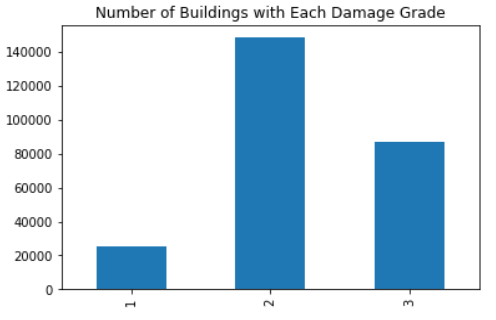
\includegraphics[width=60mm]{images/dt_figure01.png}
    \caption{Exploratory Data Analysis: Distribution of labels.}
    \label{PICTURE_figure_dt_01}
    \end{minipage}
  \hspace{0.1cm}
  \begin{minipage}[b]{0.5\linewidth}
    \centering
    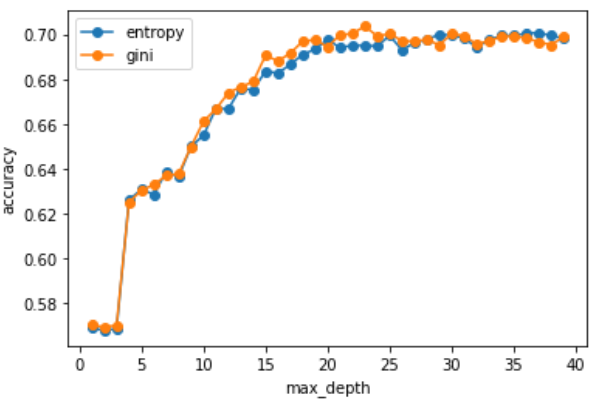
\includegraphics[width=60mm]{images/dt_figure02.png}
    \caption{Decision Trees: Manual tuning of parameters.}
    \label{PICTURE_figure_dt_02}
  \end{minipage}
\end{figure}

For the two remaining parameters, the minimum samples split and minimum samples leaf, we use the values provided from the lecturers resources, as they seem to improve the f1-score the most. With all of these parameters applied, the achieved f1-score of the classifier is 0.6966, which is worse than the score obtained by KNN.